% questions.tex —— 1990 年·全国卷·理科 · 题目内容片段（无答案）
% 由 tools/generate_projects.py 依固定源稿生成，待来源登记后重生成


\begin{gktip}
\textbf{来源说明}：固定来源为一页 A3 题面扫描，页眉印有“1990 普通高等学校招生考试（全国卷理）”，印刷页码 36。当前只认证到这个固定文件，不推断出版社、版次或官方原件身份。PDF 不含答案或解析页；后续答案和解析均为编者推导，不作官方答案。

\textbf{图形说明}：原卷第 5、11、20、23 题图形以 TikZ 矢量重绘，仅保留可见拓扑、标号和虚实线；图形不表示未给定的精确比例或度量条件，不提交页面截图。

\textbf{第 9 题符号}：原页显示 $\overline{M}\cap\overline{N}$；文本提取层会漏掉集合上划线，本稿按原页保留。

\textbf{待核（第 20 题）}：原文写两部分体积为 $V_1,V_2$，但未说明图中哪一部分对应 $V_1$ 或 $V_2$。题面照录；任何体积比方向结论须待可靠来源核清后再定。

\textbf{原文与图示差异（第 23 题）}：题干交点记作 $D$，原图标签带撇号 $D'$；题面与图稿分别照录，不推测或统一记号。
\end{gktip}

\gkpart{试题}

\gkpart{一、选择题}

\begin{question}
\gkti{1}方程 $2^{\log_3 x}=\dfrac14$ 的解是\mbox{（　　）}。

（A）$x=\dfrac19$　　（B）$x=\dfrac{\sqrt3}{3}$　　（C）$x=\sqrt3$　　（D）$x=9$

\end{question}
\begin{question}
\gkti{2}把复数 $1+i$ 对应的向量按顺时针方向旋转 $\dfrac{2\pi}{3}$，所得向量对应的复数是\mbox{（　　）}。

（A）$\dfrac{1-\sqrt3}{2}+\dfrac{-1+\sqrt3}{2}i$　　（B）$\dfrac{-1+\sqrt3}{2}+\dfrac{-1-\sqrt3}{2}i$

（C）$\dfrac{-1+\sqrt3}{2}+\dfrac{1-\sqrt3}{2}i$　　（D）$\dfrac{1-\sqrt3}{2}+\dfrac{-1-\sqrt3}{2}i$

\end{question}
\begin{question}
\gkti{3}如果轴截面为正方形的圆柱的侧面积是 $S$，那么圆柱的体积等于\mbox{（　　）}。

（A）$\dfrac S2\sqrt S$　　（B）$\dfrac S2\sqrt{\dfrac S\pi}$　　（C）$\dfrac S4\sqrt S$　　（D）$\dfrac S4\sqrt{\dfrac S\pi}$

\end{question}
\begin{question}
\gkti{4}方程 $\sin 2x=\sin x$ 在区间 $(0,2\pi)$ 内的解的个数是\mbox{（　　）}。

（A）$1$　　（B）$2$　　（C）$3$　　（D）$4$

\Needspace{0.4\textheight}
\end{question}
\begin{question}
\gkti{5}如图是函数 $y=2\sin(\omega x+\varphi)$（$|\varphi|<\dfrac\pi2$）的图象，那么\mbox{（　　）}。
\nopagebreak[4]
\begin{center}% 原卷第5题正弦曲线及坐标标记；依源图走势重绘，非截图。
\begin{tikzpicture}[x=1.35cm,y=0.72cm,line cap=round,line join=round]
  \draw[->] (-0.38,0) -- (3.45,0) node[right] {$x$};
  \draw[->] (0,-2.25) -- (0,2.25) node[above] {$y$};
  \draw[thick,domain=-0.34:3.32,samples=140,smooth,variable=\t]
    plot (\t,{2*sin(2*\t r+30)});
  \draw (-0.06,1) -- (0.06,1);
  \node[left] at (-0.06,1) {$1$};
  \node[below left] at (0,0) {$O$};
  \node[below] at (2.879793,0) {$\dfrac{11\pi}{12}$};
\end{tikzpicture}
\end{center}
\nopagebreak[4]
（A）$\omega=\dfrac{10}{11},\ \varphi=\dfrac\pi6$　　（B）$\omega=\dfrac{10}{11},\ \varphi=-\dfrac\pi6$

（C）$\omega=2,\ \varphi=\dfrac\pi6$　　（D）$\omega=2,\ \varphi=-\dfrac\pi6$

\end{question}
\begin{question}
\gkti{6}函数
\nopagebreak[4]
\[
y=\frac{\sin x}{|\sin x|}+\frac{|\cos x|}{\cos x}+\frac{\tan x}{|\tan x|}+\frac{|\cot x|}{\cot x}
\]
的值域是\mbox{（　　）}。

（A）$\{-2,4\}$　　（B）$\{-2,0,4\}$　　（C）$\{-2,0,2,4\}$　　（D）$\{-4,-2,0,4\}$

\end{question}
\begin{question}
\gkti{7}如果直线 $y=ax+2$ 与直线 $y=3x-b$ 关于直线 $y=x$ 对称，那么\mbox{（　　）}。

（A）$a=\dfrac13,\ b=6$　　（B）$a=\dfrac13,\ b=-6$

（C）$a=3,\ b=-2$　　（D）$a=3,\ b=6$

\end{question}
\begin{question}
\gkti{8}极坐标方程 $4\rho\sin^2\dfrac\theta2=5$ 表示的曲线是\mbox{（　　）}。

（A）圆　　（B）椭圆　　（C）双曲线的一支　　（D）抛物线

\end{question}
\begin{question}
\gkti{9}设全集 $I=\{(x,y)\mid x,y\in\mathbb R\}$，集合
\nopagebreak[4]
\[
M=\left\{(x,y)\ \middle|\ \frac{y-3}{x-2}=1\right\},\qquad N=\{(x,y)\mid y\ne x+1\}.
\]
那么 $\overline{M}\cap\overline{N}$ 等于\mbox{（　　）}。

（A）$\varnothing$　　（B）$\{(2,3)\}$　　（C）$(2,3)$　　（D）$\{(x,y)\mid y=x+1\}$

\end{question}
\begin{question}
\gkti{10}如果实数 $x,y$ 满足等式 $(x-2)^2+y^2=3$，那么 $\dfrac yx$ 的最大值是\mbox{（　　）}。

（A）$\dfrac12$　　（B）$\dfrac{\sqrt3}{3}$　　（C）$\dfrac{\sqrt3}{2}$　　（D）$\sqrt3$

\Needspace{0.4\textheight}
\end{question}
\begin{question}
\gkti{11}如图，正三棱锥 $S-ABC$ 的侧棱与底面边长相等，如果 $E,F$ 分别为 $SC,AB$ 的中点，那么异面直线 $EF$ 与 $SA$ 所成的角等于\mbox{（　　）}。
\nopagebreak[4]
\begin{center}% 原卷第11题正三棱锥；E,F 为 SC、AB 中点，底面后棱与 EF 用虚线。
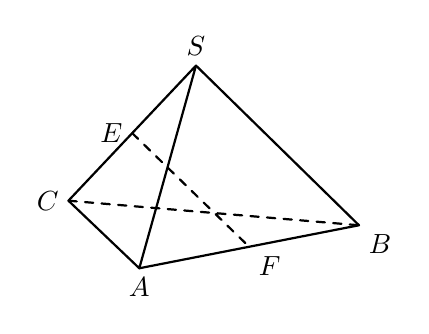
\begin{tikzpicture}[x=0.9cm,y=0.78cm,line cap=round,line join=round]
  \coordinate (S) at (0.8,3.3);
  \coordinate (A) at (0,0);
  \coordinate (B) at (3.1,0.7);
  \coordinate (C) at (-1.0,1.1);
  \coordinate (E) at (-0.1,2.2);
  \coordinate (F) at (1.55,0.35);
  \draw[thick] (S)--(A)--(C)--(S);
  \draw[thick] (S)--(B)--(A);
  \draw[thick,dashed] (C)--(B) (E)--(F);
  \node[above] at (S) {$S$};
  \node[below] at (A) {$A$};
  \node[below right] at (B) {$B$};
  \node[left] at (C) {$C$};
  \node[left] at (E) {$E$};
  \node[below right] at (F) {$F$};
\end{tikzpicture}
\end{center}
\nopagebreak[4]
（A）$90^\circ$　　（B）$60^\circ$　　（C）$45^\circ$　　（D）$30^\circ$

\end{question}
\begin{question}
\gkti{12}已知 $h>0$。设命题甲为：两个实数 $a,b$ 满足 $|a-b|<2h$；命题乙为：两个实数 $a,b$ 满足 $|a-1|<h$ 且 $|b-1|<h$。那么甲是乙的\mbox{（　　）}。

（A）充分不必要条件　　（B）必要不充分条件

（C）充要条件　　（D）既不充分也不必要条件

\end{question}
\begin{question}
\gkti{13}$A,B,C,D,E$ 五人并排站成一排，如果 $B$ 必须站在 $A$ 的右边（$A,B$ 可以不相邻），那么不同的排法共有\mbox{（　　）}。

（A）$24$ 种　　（B）$60$ 种　　（C）$90$ 种　　（D）$120$ 种

\end{question}
\begin{question}
\gkti{14}以一个正方体的顶点为顶点的四面体共有\mbox{（　　）}。

（A）$70$ 个　　（B）$64$ 个　　（C）$58$ 个　　（D）$52$ 个

\end{question}
\begin{question}
\gkti{15}设函数 $y=\arctan x$ 的图象沿 $x$ 轴正方向平移 $2$ 个单位所得到的图象为 $C$。又设图象 $C'$ 与 $C$ 关于原点对称，那么 $C'$ 所对应的函数是\mbox{（　　）}。

（A）$y=-\arctan(x-2)$　　（B）$y=\arctan(x-2)$

（C）$y=-\arctan(x+2)$　　（D）$y=\arctan(x+2)$

\end{question}
\gkpart{二、填空题}

\begin{question}
\gkti{16}双曲线 $\dfrac{y^2}{16}-\dfrac{x^2}{9}=1$ 的准线方程是\gkblank{}。

\end{question}
\begin{question}
\gkti{17}$(x-1)-(x-1)^2+(x-1)^3-(x-1)^4+(x-1)^5$ 的展开式中，$x^2$ 的系数等于\gkblank{}。

\end{question}
\begin{question}
\gkti{18}已知 $\{a_n\}$ 是公差不为零的等差数列，如果 $S_n$ 是 $\{a_n\}$ 的前 $n$ 项的和，那么
\nopagebreak[4]
\[
\lim_{n\to\infty}\frac{na_n}{S_n}
\]
等于\gkblank{}。

\end{question}
\begin{question}
\gkti{19}函数 $y=\sin x\cos x+\sin x+\cos x$ 的最大值是\gkblank{}。

\Needspace{0.4\textheight}
\end{question}
\begin{question}
\gkti{20}如图，三棱柱 $ABC-A_1B_1C_1$ 中，若 $E,F$ 分别为 $AB,AC$ 的中点，平面 $EB_1C_1F$ 将三棱柱分成体积为 $V_1,V_2$ 的两部分，那么 $V_1:V_2=$\gkblank{}。
\nopagebreak[4]
\begin{center}% 原卷第20题三棱柱及平面 EB_1C_1F；不标注未出现在原图中的体积区域名。
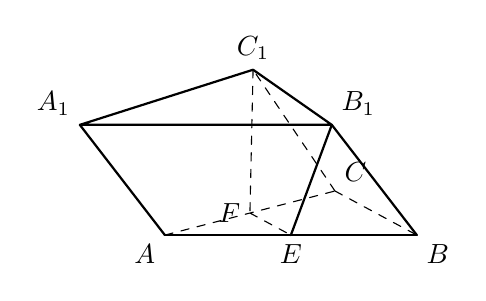
\begin{tikzpicture}[x=0.8cm,y=0.7cm,line cap=round,line join=round]
  \coordinate (A) at (0,0);
  \coordinate (B) at (4,0);
  \coordinate (C) at (2.7,0.8);
  \coordinate (Aone) at (-1.35,2.0);
  \coordinate (Bone) at (2.65,2.0);
  \coordinate (Cone) at (1.4,3.0);
  \coordinate (E) at (2,0);
  \coordinate (F) at (1.35,0.4);
  \draw[thick] (A)--(B);
  \draw[thick] (Aone)--(Bone)--(Cone)--(Aone);
  \draw[thick] (A)--(Aone) (B)--(Bone);
  \draw[dashed] (A)--(C) (C)--(Cone) (C)--(B) (Cone)--(F) (F)--(E);
  \draw[thick] (E)--(Bone);
  \node[below left] at (A) {$A$};
  \node[below right] at (B) {$B$};
  \node[above right] at (C) {$C$};
  \node[above left] at (Aone) {$A_1$};
  \node[above right] at (Bone) {$B_1$};
  \node[above] at (Cone) {$C_1$};
  \node[below] at (E) {$E$};
  \node[left] at (F) {$F$};
\end{tikzpicture}
\end{center}
\nopagebreak[4]
\end{question}
\gkpart{三、解答题}

\begin{question}
\gkti{21}有四个数，其中前三个数成等差数列，后三个数成等比数列，并且第一个数与第四个数的和是 $16$，第二个数与第三个数的和是 $12$。求这四个数。

\end{question}
\begin{question}
\gkti{22}已知 $\sin\alpha+\sin\beta=\dfrac14$，$\cos\alpha+\cos\beta=\dfrac13$，求 $\tan(\alpha+\beta)$ 的值。

\Needspace{0.4\textheight}
\end{question}
\begin{question}
\gkti{23}如图，在三棱锥 $S-ABC$ 中，$SA\perp$ 底面 $ABC$，$AB\perp BC$。$DE$ 垂直平分 $SC$，且分别交 $AC,SC$ 于 $D,E$。又 $SA=AB$，$SB=BC$。求以 $BD$ 为棱、以 $BDE$ 与 $BDC$ 为面的二面角的度数。
\nopagebreak[4]
\begin{center}% 原卷第23题三棱锥；D 按题干为 AC 上交点，原图标签按可见记号保留为 D'。
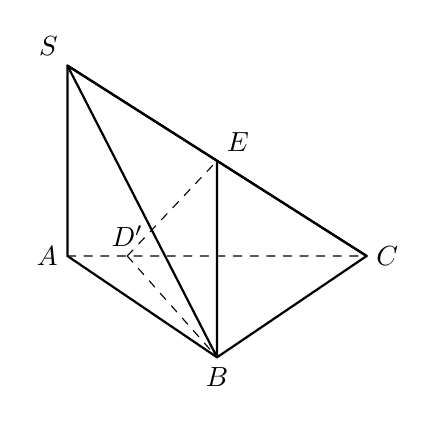
\begin{tikzpicture}[x=0.95cm,y=0.78cm,line cap=round,line join=round]
  \coordinate (A) at (-1.6,0);
  \coordinate (C) at (2.4,0);
  \coordinate (B) at (0.4,-1.65);
  \coordinate (S) at (-1.6,3.1);
  \coordinate (D) at (-0.8,0);
  \coordinate (E) at (0.4,1.55);
  \draw[thick] (A)--(S)--(C)--(B)--cycle;
  \draw[thick] (S)--(B) (S)--(E) (E)--(C) (E)--(B);
  \draw[dashed] (A)--(C) (D)--(B) (D)--(E);
  \node[above left] at (S) {$S$};
  \node[left] at (A) {$A$};
  \node[below] at (B) {$B$};
  \node[right] at (C) {$C$};
  \node[above] at (D) {$D'$};
  \node[above right] at (E) {$E$};
\end{tikzpicture}
\end{center}
\nopagebreak[4]
\end{question}
\begin{question}
\gkti{24}设 $a\ge0$，在复数集 $\mathbb C$ 中解方程：$z^2+2|z|=a$。

\end{question}
\begin{question}
\gkti{25}设椭圆的中心是坐标原点，长轴在 $x$ 轴上，离心率 $e=\dfrac{\sqrt3}{2}$。已知点 $P\left(0,\dfrac32\right)$ 到这个椭圆上的点的最远距离是 $\sqrt7$。求这个椭圆的方程，并求椭圆上到点 $P$ 的距离等于 $\sqrt7$ 的点的坐标。

\end{question}
\begin{question}
\gkti{26}$f(x)=\lg\dfrac{1+2^x+\cdots+(n-1)^x+n^x a}{n}$，其中 $a$ 是实数，$n$ 是任意自然数且 $n\ge2$。

（1）如果 $f(x)$ 当 $x\in(-\infty,1]$ 时有意义，求 $a$ 的取值范围；

（2）如果 $a\in(0,1]$，证明：$2f(x)<f(2x)$ 当 $x\ne0$ 时成立。

\end{question}